\documentclass[./../main.tex]{subfiles}

\begin{document}
\subsection{Các nút vào đầu nối}
\begin{figure}[H]
	\centering
	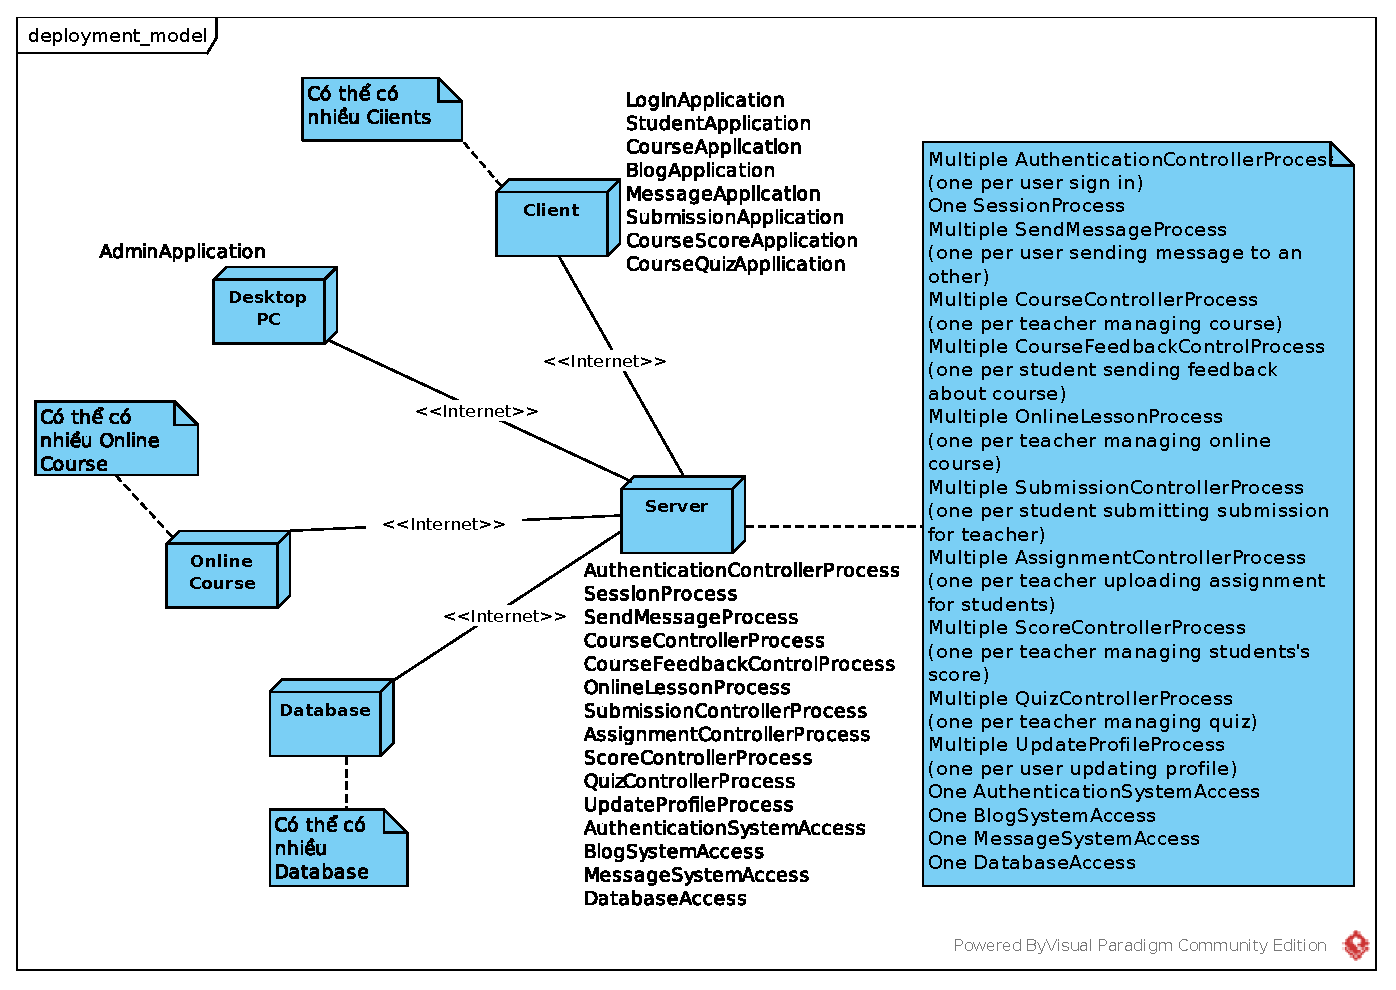
\includegraphics[width=\linewidth]{./images/deployment_model.eps}
	\caption{Các nút và đầu nối}
\end{figure}
\subsection{Ánh xạ các tiến trình vào nút}
Các tiến trình được chạy trên Client là:
\begin{itemize}
	\item LogInApplication
	\item StudentApplication
	\item CourseApplication
	\item BlogApplication
	\item MessageApplication
	\item SubmissionApplication
	\item CourseScoreApplication
	\item CourseQuizAppllication
\end{itemize}
Các tiến trình được chạy trên Desktop PC là:
\begin{itemize}
	\item AdminApplication
\end{itemize}

Các tiến trình được chạy trên Server là:
\begin{itemize}
	\item AuthenticationControllerProcess
	\item SessionProcess
	\item SendMessageProcess
	\item CourseControllerProcess
	\item CourseFeedbackControlProcess
	\item OnlineLessonProcess
	\item SubmissionControllerProcess
	\item AssignmentControllerProcess
	\item ScoreControllerProcess
	\item QuizControllerProcess
	\item UpdateProfileProcess
	\item AuthenticationSystemAccess
	\item BlogSystemAccess
	\item MessageSystemAccess
	\item DatabaseAccess
\end{itemize}

\end{document}